\newpage
\section{Dynamik}
\subsection{Newtonsche Gesetze}
\subsubsection{Erstes Newtonsches Gesetz Trägheitsgesetz}
Ein Körper verharrt im Zustand der Ruhe oder der gleichförmigen Bewegung, wenn er
nicht durch einwirkende Kräfte gezwungen wird, seinen Zustand zu ändern. Die Gesamt-
summe der Kräfte in einem abgeschlossenen System ist unveränderlich:

\subsubsection{Zweites Newtonsches Gesetz (Aktionsgesetz)}
Die Beschleunigung eines Körpers ist umgekehrt proportional zu seiner Masse und direkt
proportional zur Kraft, die auf ihn wirkt.

\subsubsection{Drittes Newtonsches Gesetz (Actio = Reactio)}
Wirkt ein Körper A auf einen Körper B mit der Kraft ~F AB , so wirkt der Körper B mit der
entgegengesetzt gerichteten, gleich grossen Kraft $\overrightarrow{F}_{BA}$.

\subsubsection{Allgemeines Vorgehen beim Lösen von Bewegungsproblemen}
\begin{enumerate}
	\item Zeichnung anfertigen
	\item Für jeden Körper, der untersucht werden soll, wird ein Kräftediagramm eingezeichnet
	\item Ein geeignetes Koordinatensystem einführen
	\item  Das entstandene Gleichungssystem aufl"osen
	\item  Ergebnisse mit gesundem Menschenverstand aufl"osen
\end{enumerate}

$F_{G} = Gewichtskraft$
$F_{R} = Reibungskraft$
$F_{N} = Normalkraft$
$\mu_{G} = Gleitreibung$
$\mu_{H} = Haftreibung$
$W_{B} = Beschleunigungsarbeit$
$E_{kin} = Kinetische Energie$

\subsubsection{Spezielle Kräfte, Masse, Dichte, Reibung}
$F_{G} = mg$ \\
$F_{R} = \mu_{G}F_{N}$ \\
$\rho = \frac{m}{V}$ \\
$\mu = - \frac{a}{g}$ \\
$\mu_{H} = \tan{}$ \\
$F_{H_{max}} = \mu_{H}F_{H}$ \\ 
\adjustbox{width=2.5cm}{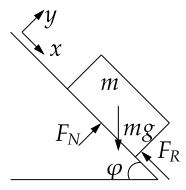
\includegraphics{bilder/spezK}}

\subsubsection{Arbeit und Energie, Energieerhaltung}
Energie ist die Fähigkeit Arbeit zu leisten. Arbeit = überwinden eines Widerstandes \\
Energie kann weder verschwinden, noch aus dem Nichts entstehen. 
Wenn gelegentlich davon gesprochen wird, dass Energie 
”vernichtet“ werde, so ist damit gemeint, dass mechanische Energie 
(potentielle oder kinetische Energie) durch Reibungsarbeit in 
”Wärme“, genauer gesagt, in innere Energie, umgewandelt wird. \\
Die Gesamtenergie eines abgeschlossenen Systems ist 
unveränderlich. \\
$dW = \overrightarrow{F} \cdot \overrightarrow{ds}$
$W = Pt$
$F = \frac{P}{v}$

\subsubsection{Leistung}

$P = \frac{\Delta W}{\Delta t} = \frac{\overrightarrow{F} \Delta \overrightarrow{s}}{ \Delta t} = \overrightarrow{F} \cdot \frac{\Delta \overrightarrow{s}}{\Delta t} = \overrightarrow{F} \cdot \overrightarrow{v} = \overrightarrow{M} \cdot \omega$ \\
Umwandlung von $1 kWh = 3.6 \cdot 10^3 J $ (Überprüfen) \\
1 PS = 735.5 W


\subsubsection{Hubarbeit, Potentielle Energie}

Potentielle Energie $E_{pot} = m \cdot g \cdot h$ \\
$W_{H} \cdot \overrightarrow{F} \cdot \overrightarrow{h}$ \\
Hubarbeit: $W_{H} = E_{pot}$

\subsubsection{Spannarbeit, Spannenergie}
Spannenergie: $E_{s} = \frac{c \cdot x^2}{2}$  entspricht Spannarbeit: $W_{s} = \overrightarrow{F_{s}} \cdot \overrightarrow{x}$ \\
$F_{F}$ = Spannkraft = $c \cdot \Delta s$ \\
x: = Spannweg [m], c: = Federkonstante


\subsubsection{Beschleunigungsarbeit, Kinetische Energie}
$E_{kin} = \frac{mv^2}{2}$
$W_{B} = \frac{m(\Delta v)^2}{2}$

\subsubsection{Rotationsenergie}
$E_{rot} = \frac{1}{2}Jw^2$

\subsubsection{Reibungsarbeit}
$W_{R} = F_{RS}$

\subsubsection{Verformungsarbeit}
$Inelatisch: W_{D} = \frac{m_{1}m_{2}(v_{1} + v_{2})^2}{2(m_{1} + m_{2})} $ \\
$Elatisch:  W_{D} = \frac{F_{1} + F_{2}}{2}\Delta s$
\adjustbox{width=2.5cm}{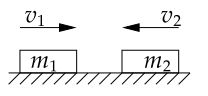
\includegraphics{bilder/verformung}}
\subsubsection{Kernbindungenergie (Einstein)}
$E = m \cdot c^2$

\subsubsection{Leistung}
$P = \frac{dW}{dt} = \frac{Fds}{dt} =\overrightarrow{F} \cdot \overrightarrow{s} = M \cdot \omega$

\subsubsection{Wirkungsgrad}
Beachte: Wo wird die Systemgrenze gezogen?! Wird z.B. die Wärmeleistung weiterverwendet? \\
Wirkungsgrad: $\eta = \frac{P_{ab}}{P_{zu}} = \frac{W_{ab}}{W_{zu}}$ \\
$\eta_{tot} = \eta_{1} \cdot \eta_{2}  \cdot ...$

\subsubsection{Impuls, Impulserhaltung}
In einem abgeschlossenen System bleibt der Gesamtimpuls konstant. 

Impuls $ \overrightarrow{p} = m \cdot \overrightarrow{v} = \overrightarrow{F}$  \\
Gesamtimpuls: $ p_{ges} = \Sigma_{i = 1} m_{i}v_{s} $\\
Kraftstoss: $\overrightarrow{F} = \frac{\Delta \overrightarrow{p}}{ \Delta t}$

\subsubsection{Drehimpuls}
Drehimpuls: $L = m \cdot v \cdot r \cdot \sin{\phi} = J \cdot \omega$ \\
$\overrightarrow{L} = \overrightarrow{r} \times \overrightarrow{p}$ \\
Drehmoment: $ \overrightarrow{M} = \frac{d \overrightarrow{p}}{dt}
$

\subsubsection{Raketenantrieb}
$v = u \cdot ln(\frac{m_0}{m} + v_0) $ \\
Schubkraft: $F_s = \frac{dm}{dt} u$ \\
Spezifischer Impuls: $T = \frac{u}{g}$
u = v-Strahl relativ zur Rakete\\ 
\adjustbox{width=2.5cm}{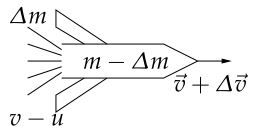
\includegraphics{bilder/raketenantrieb}}

\subsection{Stösse}

\begin{tabular}[c]{|l|l|}
	\hline
	Stossart & Beschreibung \\
	\hline
	gerade & Die Bahnen der Schwerpunkte liegen auf einer Geraden. \\
	\hline
	schief & Die Bahnen der Schwerpunkte schliessen einen Winkel ein. \\
	\hline
	zentral & Die Schwerpunkte der Stosspartner liegen auf der Strossnormalen.  \\
	\hline
	exzentrisch & Die Schwerpunkte der Stosspartner liegen nicht auf der Strossnormalen.  \\
	\hline
	elastisch & Die totalen kinetischen Energien vor und nach dem Stoss sind gleich.  \\
		\hline
	inelastisch & Die totalen kinetischen Energien vor und nach dem Stoss sind verschieden.  \\
	\hline
	total inelastisch & Die Stosspartner bewegen sich nach dem Stoss mit der gleichen Geschwindigkeit.  \\
	\hline
\end{tabular}

%
%	\adjustbox{width=15cm}{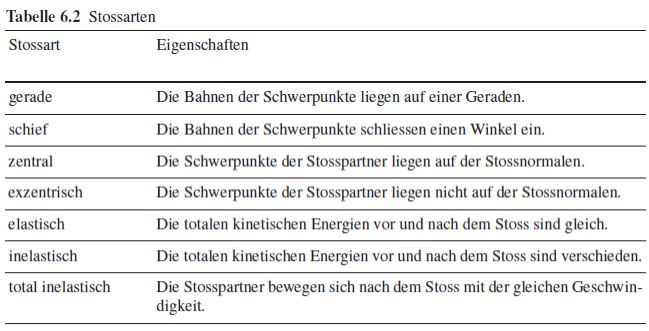
\includegraphics{bilder/Stossarten}}

\subsubsection{Inelastischer Stoss}
Bei einem inelatischen Stoss geht ein Teil der kinetischen Energie als Wärmeenergie "verloren". \\
$v' = \frac{m_1v_1 + m_2v_2}{m_1 + m_2}$ \\
$Q = \frac{u \cdot v_{R}^2}{2} = \frac{m_1 \cdot m_2}{m_1 + m_2} \cdot \frac{1}{2}(v_1 - v_2) $

\subsubsection{Elastischer Stoss}
Bei einem elastischen Stoss bleibt die kinetische Energie als auch der Impuls erhalten. \\
Achtung: Wird etwas auf den Boden geschleudert und kommt wieder zurück: 2 x $E_kin$

$v_1 - v_2 = -(v'_1 - v'_2)$ \\
$v'_1 = \frac{(m_1 - m_2)v_1 + 2m_2v_2}{m_1 + m_2} $ \\
$v'_2 = \frac{(m_2 - m_1)v_2 + 2m_1v_1}{m_1 + m_2}$ \\
Impulserhaltung: $m_1v_1 + m_2v_2 = m_1v'_1 + m_2v'_2$ \\
Energieerhaltung: $m_1v_1^2 + m_2v^2_2 = m_1v_1^{'2} + m_2v_2^{'2}$ \\
$v'$ = Geschwindigkeit nach dem Stoss \\

\section{Gravitationsgesetze}
\begin{multicols}{3}
\textbf{1. Kepler Gesetz} \\
Die Planeten bewegen sich auf Elipsen, in deren einen Brennpunkt die Sonne steht. \\
\adjustbox{width=2.5cm}{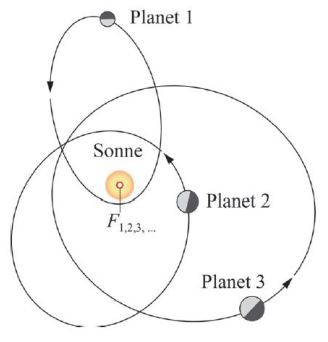
\includegraphics{bilder/kepler1}}
\columnbreak

\textbf{2. Kepler Gesetz} \\
Der Fahrstrahl des Planeten überstreicht in gleichen Zeiten gleiche Flächen. \\
\\
\adjustbox{width=3.5cm}{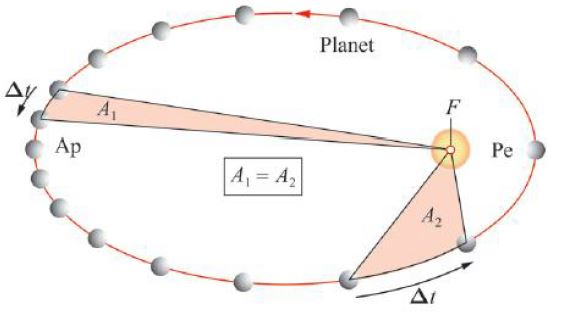
\includegraphics{bilder/kepler2}}
\columnbreak

\textbf{3. Kepler Gesetz} \\
Die Quadrate der Umlaufzeiten zweier Planeten verhalten sich wie Kuben der Halbachsen ihrer Bahnen. \\
\\
$$a_2 = (\frac{T_1}{T_2})^\frac{2}{3} \cdot a_1 $$ \\
\end{multicols}

\textbf{Newtonsche Gravitationsgesetze:} \\
$ F_G = G\frac{m_1 \cdot m_2}{r^2} $ \\
Gravitationskonstante G: $6.673 \cdot 10^{-11} m^3 / kg s^2$
